\chapter{Anteproyecto}

\section{Descripción y Alcance del proyecto}
\subsection{Antecedentes}
El proyecto es solicitado por Komuness CR, una organización comunitaria dedicada a promover proyectos que fortalezcan el desarrollo social, cultural y educativo en comunidades en situación de vulnerabilidad, como el barrio de Tejarcillos en Alajuelita. Komuness CR se integró a la estructura de Coopesinergía, una cooperativa autogestionaria que realiza proyectos orientados al desarrollo humano integral, principalmente en comunidades con menor acceso a recursos básicos (P. Monge, comunicación personal, 18 de agosto de 2025).

La necesidad que motiva este proyecto es la marcada brecha social y tecnológica que limita las oportunidades de desarrollo de los habitantes de Tejarcillos, especialmente de los jóvenes. Esta población carece de espacios y recursos adecuados para exponer sus talentos, productos y servicios, lo que reduce su participación en actividades culturales, educativas y económicas (P. Monge y T. Chaverry, comunicación personal, 18 de agosto de 2025).

El proyecto solventará esta necesidad mediante el desarrollo de una plataforma digital que servirá como espacio para que los jóvenes y vecinos de Tejarcillos puedan compartir sus productos, servicios y eventos culturales, además de contar con una biblioteca digital donde se registren proyectos y materiales de interés. El impacto esperado es el fortalecimiento del empoderamiento juvenil, la inclusión tecnológica y la participación cultural.

Los beneficios del proyecto alcanzarán principalmente a los jóvenes y habitantes del barrio Tejarcillos en Alajuelita, cuyo estilo de vida podrá mejorar al contar con herramientas digitales que fomenten la inclusión y la equidad, brindando espacios para visibilizar y registrar proyectos culturales y comunitarios.

\subsection{Objetivos}

%
% Los objetivos del proyecto deben englobar el alcance total. Todo objetivo debe estar redactado respetando la siguiente estructura:

% Verbo infinitivo: Representa una acción que el equipo de desarrollo ejecutará durante el proyecto. Debe ser una acción concreta y relevante para completar el proyecto

% Objeto: Indica el objeto sobre el cual se aplicará la acción. Típicamente representa el producto esperado de la acción

% Modo: Indica parámetros por los cuales se medirá la calidad y completitud del resultado. 

% Ejemplo: Desarrollar un sistema de facturación electrónica que provea una interfaz amigable para el usuario y cumpla con los estándares impuestos por el Ministerio de Hacienda de Costa Rica. 

% Sólo puede existir un verbo infinitivo en el objetivo
% Debe ser posible medir el nivel de cumplimiento del objetivo, es decir, debe ser posible decir en cualquier momento del proyecto, cual porcentaje del objetivo se ha cumplido.

\begin{itemize}
    \item \textbf{Objetivo General}
    \begin{itemize}
        \item Desarrollar una plataforma digital para la comunidad juvenil de Alajuelita que visibilice sus talentos y servicios culturales mediante una biblioteca digital, mejore el sistema de publicaciones y garantice su sostenibilidad con un sistema de membresías premium, utilizando el stack tecnológico MERN e integrando APIs de PayPal para transacciones seguras.

    \end{itemize}
    \item \textbf{Objetivos Específicos}
    \begin{itemize}
        \item Optimizar el módulo de publicaciones y eventos de la plataforma que facilite la consulta y gestión de la información comunitaria, implementando un sistema de categorías, un calendario interactivo y un servidor para archivos.
         \item Integrar un sistema de usuarios premium y pagos mediante PayPal que permita la monetización de membresías, configurando límites de publicaciones y flujos de transacción.
        \item Integrar perfiles públicos y un banco de profesionales que facilite la búsqueda de talentos que forman parte de la comunidad.
    \end{itemize}
\end{itemize}

\subsection{Involucrados}
% Liste los diferentes involucrados en este proyecto, incluya en una figura un organigrama en el cual se ilustre la relación entre todos los participantes e interesados con los miembros del equipo de trabajo.

\begin{table}[H]
\caption{Involucrados en el proyecto}
\label{tab:involucrados}
\centering
\small
\begin{tabular}{|l|l|l|}
\hline
\textbf{Nombre del involucrado} & \textbf{Rol} & \textbf{Contacto} \\
\hline \hline
Rodolfo Mora Zamora & Supervisor - Profesor TEC & rodmora@itcr.ac.cr \\
\hline
Paola Monge & Cliente - Directora Fondo Inés Revueltas & komunesscr@gmail.com \\
\hline
Tatiana Chaverry & Cliente - Coordinadora Grupo Jóvenes Komuness & komunesscr@gmail.com \\
\hline
Fredrik Aburto Jiménez & Desarrollador - TEC & fredrik@estudiantec.cr \\
\hline
Angélica Díaz Barrios & Desarrolladora - TEC & diazbarrios2001@estudiantec.cr \\
\hline
Andrés Salas Araya & Desarrollador - TEC & asaraya153@estudiantec.cr \\
\hline
\end{tabular}
\caption{Lista de involucrados y sus contactos}
\end{table}

% Organigrama
\begin{figure}[H]
  \centering
  \begin{tikzpicture}[
      node distance=1.5cm and 2cm,
      every node/.style={rectangle, rounded corners, draw, align=center, minimum width=3cm, fill=blue!10},
      arrow/.style={->, thick, >=stealth}
    ]
    
    % Nodo supervisor
    \node (supervisor) [fill=red!20] {Supervisor\\Rodolfo Mora Zamora\\\small{Profesor TEC}};
    
    % Nodo cliente
    \node (cliente) [right=of supervisor, fill=green!20] {Cliente\\Komuness CR\\\small{P. Monge - T. Chaverry}};
    
    % Equipo de desarrollo
    \node (equipo) [below=2cm of supervisor, fill=yellow!20] {Equipo de Desarrollo\\Tecnológico de Costa Rica};
    
    % Desarrolladores
    \node (dev1) [below left=of equipo] {Fredrik Aburto Jiménez\\\small{Desarrollador}};
    \node (dev2) [below=of equipo] {Angélica Díaz Barrios\\\small{Desarrolladora}};
    \node (dev3) [below right=of equipo] {Andrés Salas Araya\\\small{Desarrollador}};
    
    % Líneas de conexión
    \draw[arrow] (supervisor) -- (equipo);
    \draw[arrow] (cliente) -- (equipo);
    \draw[arrow] (equipo) -- (dev1);
    \draw[arrow] (equipo) -- (dev2);
    \draw[arrow] (equipo) -- (dev3);
    
    % Línea de supervisión cliente
    \draw[dashed, arrow] (supervisor) to [bend left=15] (cliente);
    
  \end{tikzpicture}
  \caption{Organigrama de la estructura del equipo e involucrados del proyecto}
  \label{fig:organigrama}
\end{figure}

\subsection{Estructura de Desglose de Trabajo}

%Divida su proyecto en cuatro Productos Mínimos Viables (MVP por sus siglas en inglés),  cada MVP debe descomponerlo en entregables que deberá presentar a su cliente al final de cada iteración. Describa cada MVP en esta sección, indicando en cuáles subproductos se divide.

%Diagrame sus entregables en una Estructura de Desglose de Trabajo (EDT) que le facilite llevar un registro de cuáles se deben cumplir en cada etapa del proyecto. Utilice esta guía para orientarse en cómo desarrollar su EDT: https://formulaproyectosurbanospmipe.wordpress.com/2012/05/09/tema-n-5-la-estructura-de-desglose-del-trabajo-edt-segun-la-guia-del-pmbok-30-04-2012-sesion-10-segunda-parte/.

% EDT
\begin{figure}[H]
  \centering
    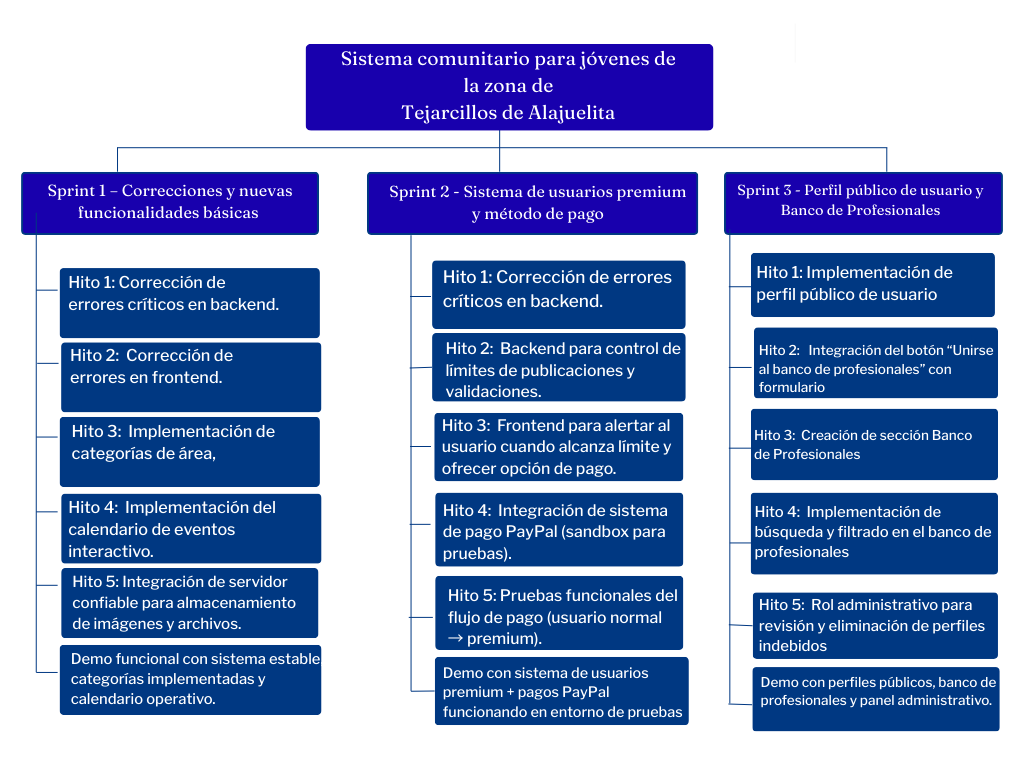
\includegraphics[height= 10cm, width=15cm]{project/images/EDT1.png}
  \caption{\textbf{Diagrama del alcance del proyecto dividido en sprints}}
\end{figure}
